\documentclass[14pt]{article}
\usepackage{url}
\usepackage{hyperref}
\usepackage{amsmath}
\usepackage{mathtools}
\usepackage{extsizes}
\usepackage{titling}
\usepackage{siunitx}
\usepackage{graphicx}
\usepackage[shortlabels]{enumitem}
\usepackage[margin=0.75in]{geometry}
\usepackage{indentfirst}
\usepackage{caption}

\newcommand{\bd}{\textbf}

\setlength{\droptitle}{-5em} 

\title{Exam 3}
\author{Mitchell Meier}
\date{\today}

\begin{document}

\maketitle

\subsection*{Problem 1}

\begin{enumerate}

\item
\begin{enumerate}[(a)]
\item
$H_0: \mu = 0.4$ \\
$H_1: \mu > 0.4$ 

\item

Significance level (p-value) $= 0.0001$ \\

$0.0001 < 0.01$, $p < \alpha$ \\

Therefore, we reject the null hypothesis $H_0$, and can say with 99\% confidence that $\mu > 0.4$, or that the proportion of adults who live in Tempe, Arizona, who are college graduates is greater than 40\%

\begin{figure}[h]
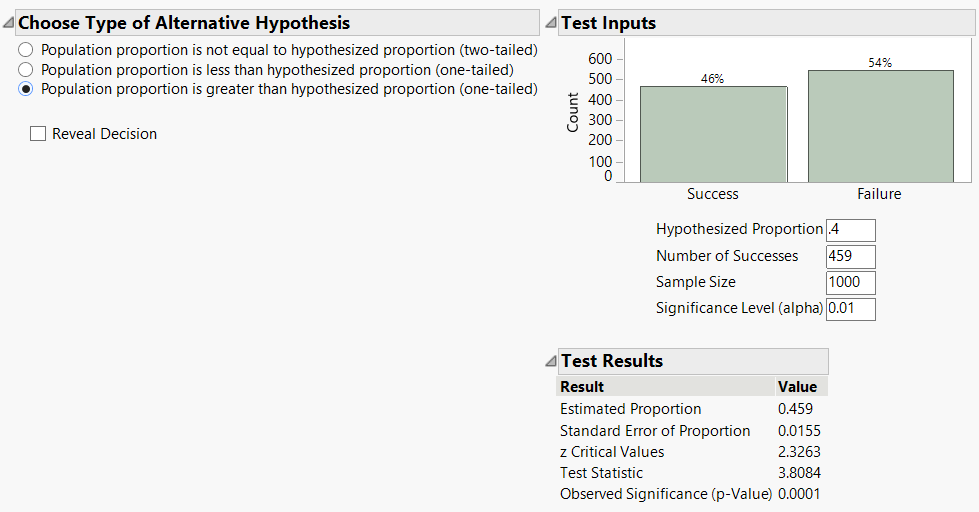
\includegraphics[scale=0.75]{exam3Pics/1-1-b.PNG}
\centering
\end{figure}

\end{enumerate}

\pagebreak

\item
\begin{enumerate}[(a)]
\item
$\mu_0 =$ Mean of weight percent calcium in standard cement \\
$\mu_1 =$ Mean of weight percent calcium in cement doped with lead \\

$H_0: \mu_1 = \mu_2$ \\
$H_1: \mu_1 > \mu_2$  



\item

When the $\alpha$ value is not given, we assume $\alpha = 0.05$ \\

Significance level (p-value) $= 0.1543$ \\

$0.1543 > 0.05$, $p > \alpha$ \\

Therefore, we fail to reject the null hypothesis $H_0$ and can not say with 95\% confidecne that the mean of weight percent calcium in standard cement is greater than the mean of weight percent calcium in cement doped with lead

\begin{figure}[h]
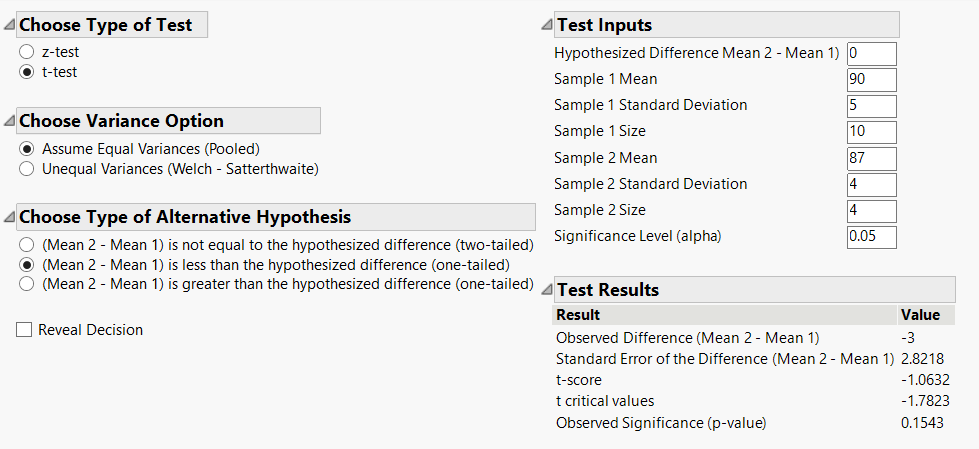
\includegraphics[scale=0.75]{exam3Pics/1-2-b.PNG}
\centering
\end{figure}

\end{enumerate}

\pagebreak

\item
\begin{enumerate}[(a)]
\item
$\mu_0 =$ the mean of the diameter of the rods produced by machine 1 \\
$\mu_1 =$ the mean of the diameter of the rods produced by machine 2 \\

$H_0: \mu_1 = \mu_2$ \\
$H_1: \mu_1 \ne \mu_2$  

\item

Significance level (p-value) $= 0.8184$ \\

$0.8184 > 0.05$, $p > \alpha$ \\

Therefore, we fail to reject the null hypothesis $H_0$ and can not say with 95\% confidecne that the mean of the diameter of the rods produced by machine 1 is different than the mean of the diameter of the rods produced by machine 2

\begin{figure}[h]
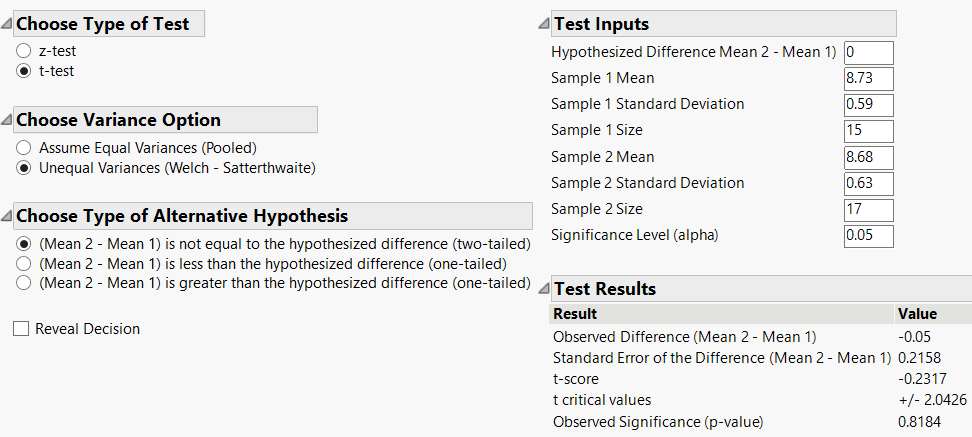
\includegraphics[scale=0.75]{exam3Pics/1-3-b.PNG}
\centering
\end{figure}

\end{enumerate}
\end{enumerate}
\pagebreak

\subsection*{Problem 2}
\begin{enumerate}
\item
The S\&P 500, or the "Standard \& Poor" 500 is a stock market index that includes all the stocks of the (roughly) top 500 United States corporations. Being a list of the top 500 companies, the S\&P 500 is a good representation of the overall United States stock market performance \\
The S\&P 500 was concieved by two financial companies, Standard and Poor, and was officially introduced on March 4th, 1957. In present day, the S\&P Dow Jones Indicies own it, and they are a joint venture between the companies McGraw Hill Financial, CME Group, and News Corp \\
To qualify to be in the S\&P index, a company must be located in the United States, have a market cap of at least 8.2 billion US dollars, have at least 50\% of its stock open to the public, have stock priced at at least 1 dollar per share, have at least 4 consecituve quarters of positive earnings, and have 50\% of its assets located in the United States \\
The S\&P tracks the market capitalization of companies in its index, which is calculated by taking the number of shares distributed by the company and multiplying it by its stock price. The companies proportion of market cap compared to the other companies in the index will determine how much representation they recievce in the index

\item

\pagebreak

\begin{enumerate}[(a)]
\item
Scatterplot Matrix of the sample data

\begin{figure}[h]
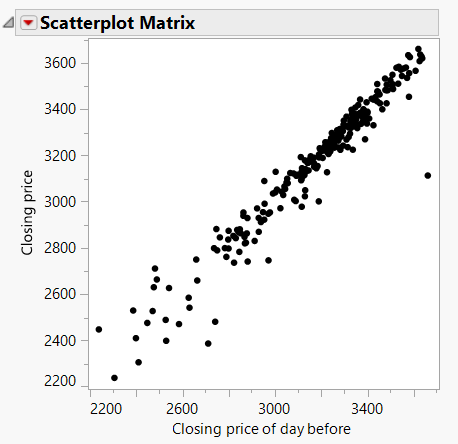
\includegraphics[scale=0.75]{exam3Pics/2-2-a.PNG}
\centering
\end{figure}

\item
Check the assumption that population distributions are normal:
\begin{figure}[h]
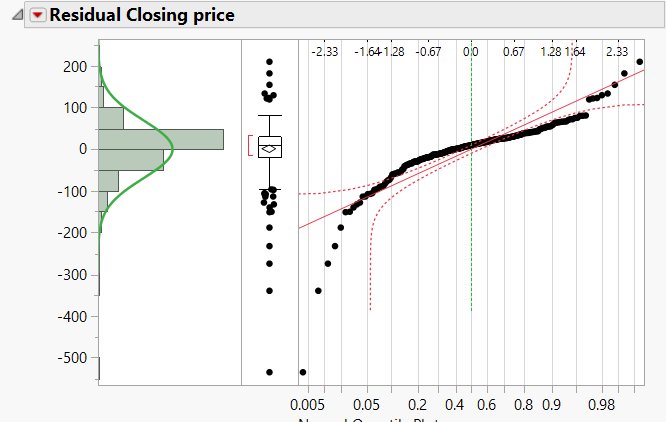
\includegraphics[scale=0.75]{exam3Pics/2-2-b-1.PNG}
\centering
\end{figure}

Shape of the distrubution resembles the shape of a normal distribution in the histogram, therefore making it safe to assume that the populations follow a normal distribution 

\pagebreak

Check the assumption that the population distributions have the same variance:
\begin{figure}[h]
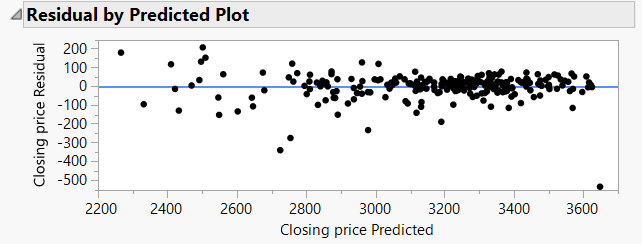
\includegraphics{exam3Pics/2-2-b-2.PNG}
\centering
\end{figure}

Residual plot values average out to around 0 and the residual plot shows no increasing or decreasing relations, therefore making it safe to assume that the populations have the same variance 

\vspace{1em}

\item
$\hat{y} = \hat{B_0} + \hat{B_1}x$ \\
$B_0 =$ Y intercept , $B_1 =$ scalar value, $x = $ closing price of day before

\item

$B_0 = 96.127$ , $B_1 = 0.9697$ \\

$\hat{y} = 96.127 + 0.9697x$


\begin{figure}[h]
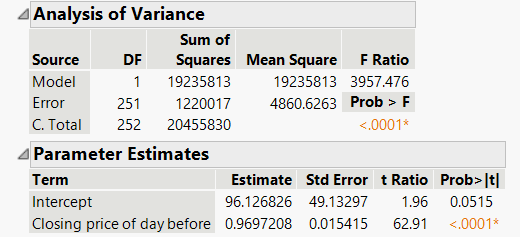
\includegraphics[scale=1.25]{exam3Pics/2-2-b-3.PNG}
\centering
\end{figure}

\end{enumerate}
\pagebreak

\item
Closing price $= x = 3662.449951$ \\

Simple Linear Regression Model: \\
$\hat{y} = 96.127 + 0.9697 \times 3662.449951$ \\
$\hat{y} = 3647.604717485$ \\

If the closing price on December 1st was \$3662.45, then the closing price the next day, December 2nd, would be \$3647.60 

\item
Yes, this does seem like an accurate model to trust when predicting the closing price of the S\&P 500 index if we know the closing price of the day before. The sample data we tested was a large sample size, seemed to follow a pattern when looking at its scatter plot, followed the assumptions of ANOVA, and produced a very small p value, all which suggests the model is accurate to not only the sample data but the population data as well



\end{enumerate}


\end{document}